\documentclass[a4paper,12pt]{article}
\usepackage{amsmath,amsfonts,amssymb} % Math packages
\usepackage{mathtools} % For defining floor and ceiling functions
\usepackage{amsthm}    % Theorems
\usepackage{bm} 	     % Bold math
\usepackage{bbm}	     % More bold math?
\usepackage{array}     % Better tables
\usepackage{chemfig}   % chemical figures
\usepackage{physics}   % derivatives and partials
\usepackage{float}     % Better positioning [H]
\usepackage{framed}    % Framed boxes
\usepackage{tcolorbox} % Colored boxes
\usepackage{geometry}  % Required for adjusting page dimensions and margins
\usepackage{graphicx}  % Include images
\usepackage{multirow}  % multicolumn tables
\usepackage{pgfplots}  % Create plots in latex
\usepackage{siunitx}   % SI unit system
\usepackage{listings}  % Code environments
\usepackage[shortlabels]{enumitem} %lets us change the enumeration to (a), (b), ...
\usepackage{booktabs}  % Better looking horizontal rules
\usepackage{makecell}  % Pre-formatting of column heads
\usepackage{hyperref}  % Clickable links
\usepackage{tikz}      % Graphs
\usetikzlibrary{shapes,arrows,positioning} % Graph arrows
\usetikzlibrary{automata,positioning,fit,shapes.geometric,backgrounds} % Node grouping
\renewcommand{\arraystretch}{1.6}

\theoremstyle{definition}
\newtheorem{definition}{Definition}[subsection]
\newtheorem{theorem}{Theorem}[subsection]
\newtheorem{lemma}{Lemma}[subsection]
\newtheorem{proposition}{Proposition}[subsection]
\pgfplotsset{width=10cm,compat=1.9}

% stats commands
\newcommand{\E}{\mathbb{E}}
\newcommand{\Var}{\mathbb{V}\mathrm{ar}}
\newcommand{\Cov}{\mathbb{C}\mathrm{ov}}
\newcommand{\Risk}{\mathcal{R}}

% common number sets
\newcommand{\N}{\mathbb{N}}
\newcommand{\R}{\mathbb{R}}
\newcommand{\Q}{\mathbb{Q}}
\newcommand{\Z}{\mathbb{Z}}
\newcommand{\C}{\mathbb{C}}

% Cs stuff
\newcommand{\bigO}{\mathcal{O}}

% Indicator function
\newcommand{\Ind}[1]{\mathbbm{1}_{\{#1\}}}

\DeclarePairedDelimiter\ceil{\lceil}{\rceil}
\DeclarePairedDelimiter\floor{\lfloor}{\rfloor}
\DeclarePairedDelimiter\angleb{\langle}{\rangle}

\geometry{
	paper=a4paper, % Paper size, change to letterpaper for US letter size
	top=2.5cm, % Top margin
	bottom=2.5cm, % Bottom margin
	left=2.5cm, % Left margin
	right=2.5cm, % Right margin
	headheight=14pt, % Header height
	footskip=1.5cm, % Space from the bottom margin to the baseline of the footer
	headsep=1.2cm, % Space from the top margin to the baseline of the header
}

\lstset{
	basicstyle=\ttfamily,
	mathescape,
	inputencoding=utf8,
	escapeinside={\%*}{*)},
	literate={á}{{\'a}}1 {ã}{{\~a}}1 {é}{{\'e}}1 {É}{{\'E}}1 {è}{{\`e}}1 {à}{{\`a}}1,
	numbers=left,
	breaklines=true
}

\let\tss\textsuperscript % superscript macro
\let\oldtextbf\mathbf
\renewcommand{\mathbf}[1]{\oldtextbf{\boldmath #1}}

\begin{document}

\title{An Introduction to Markov Chains}
\author{David Zhao}
\date{May 20, 2022}
\maketitle
\pagenumbering{arabic}

\section*{Introduction}

In the year 1906, Russian mathematician Andrey Markov published his first paper
introducing a probabilistic model that analyses sequences of events, 
which would later be designated as \emph{Markov chains} or \emph{Markov Processes}. His work has been extensively employed
in many important fields such as Natural Language Processing (NLP), PageRank, speech recognition, robot localization, etc.

\section{Markov Chain}

	A Markov chain describes a discrete-time stochastic process that consists of a finite (or infinite) set of states, 
	which is also known as a \emph{state space}. Initially, the process begins at any 
	one of these states and then successively "steps" from one state to another according to some probability known as 
	a \emph{transition probability}. If the process is currently at state $i$, then we denote the probability 
	that it transitions to state $j$ in one step as $p_{ij}$.
	\newline
	Furthermore, consider a sequence of random variables $\mathbf{X} = \{X_n \in S | n \in T\}$ where $T$ is a discrete time index 
	set. Then wey say $\mathbf{X}$ is a Markov chain if and only if, at any given time $n$, the conditional probability distribution for future states
	of the process depends only on the present state and not past states. In mathematical notation, this memoryless
	property can be expressed as

	\begin{equation*}
		\begin{aligned}
			p_{ij} = P(X_{n+1} = j | X_{n} = i, X_{n-1}, ... , X_0) = P(X_{n+1} = j | X_{n}= i)
		\end{aligned}
	\end{equation*}

	This is formally known as the \emph{Markov property} or \emph{Markov assumption}
	
\subsection{Time Homogeneity}
	
	An important assumption that we impose on Markov chains is that the conditional probability 
	distribution of $X_{n+1}$ given $X_n$ is \emph{independent} of the time $n$. Hence, for any state $i,j \in S$, and time index $n \in T$,
	the following time-invariant property holds.
	\begin{equation*}
		\begin{aligned}
			p_{ij} = P(X_{n+1} = j | X_{n} = i)
		\end{aligned}
	\end{equation*}
	In contrast, processes whose transition probabilities do depend on the time index $n$ are called \emph{time-inhomogenous}.
	For our purposes, we will only focus on \emph{time-homogeneous} processes.
	
\subsection{Transition Probabilities}
	
	For a single-step transition, recall that the probability of moving from state $i$ to $j$ is denoted as $p_{ij}$. 
	However, this notation quickly becomes strenuous if we wish to determine the evolution of the process after 2 or more
	steps. For that reason, we introduce a parameter $n$ where $p_{ij}(n)$ denotes the n-step transition 
	probability, that is, the probability of moving from state $i$ to $j$ in exactly \emph{n} steps. 
		
	\[p_{ij}(n) = P(X_{n} = j | X_{0} = i)\]
	
	For example, consider a Markov chain with state space $S = \{s_1, s_2, s_3\}$ which starts at $s_1$. If we wish 
	to determine the probability of moving to $s_3$ in exactly 2 steps, then, by the law of total probability, we must consider 
	every possible route from $s_1$ to $s_3$.

	\begin{figure}[h]
		\centering
		\tikzstyle{level 1}=[level distance=3.5cm, sibling distance=2.5cm]
		\tikzstyle{level 2}=[level distance=3.5cm]
		\tikzstyle{bag} = [text width=4em, text centered]
		\tikzstyle{end} = [circle, minimum width=3pt,fill, inner sep=0pt]
		\begin{tikzpicture}[grow=right, sloped]
		\node[bag] {$s_1$}
			child {
				node[bag] {$s_3$}        
					child {
						node[end, label=right:
							{$s_3$}] {}
						edge from parent
						node[below] {$p_{33}$}
					}
					edge from parent 
					node[below]  {$p_{13}$}
			}
			child {
				node[bag] {$s_2$}        
				child {
						node[end, label=right:
							{$s_3$}] {}
						edge from parent
						node[above] {$p_{23}$}
					}
				edge from parent         
					node[above] {$p_{12}$}
			}
			child {
				node[bag] {$s_1$}        
					child {
						node[end, label=right:
							{$s_3$}] {}
						edge from parent
						node[above] {$p_{13}$}
					}
					edge from parent 
					node[above] {$p_{11}$}
			};
		\end{tikzpicture}
		\caption{Probability Tree Diagram of Routes From $s_1$ to $s_3$}
	\end{figure}

	As such, the probability of moving from $s_1$ to $s_3$ in 2 steps is
	
	\begin{equation}
		\begin{aligned}
			p_{13}(2) = p_{11}p_{13} + p_{12}p_{23} + p_{13}p_{33}
		\end{aligned}
	\end{equation}

		
	Notice that the above equation is closely related to a dot product between two probability vectors. To make better use
	of this observation, we introduce some notation. Let $m = |S|$, then we define the \emph{transition matrix} $\mathbf{P} \in \R^{m \times m}$
	where the $(i,j)$ entry corresponds to the transition probability $p_{ij}$. In our example, the \emph{transition matrix} is written as
	
	\begin{equation*}
		\mathbf{P} = 
		\begin{pmatrix}
			p_{11} & p_{12} & p_{13} \\
			p_{12} & p_{22} & p_{23} \\
			p_{13} & p_{32} & p_{33} \\
		\end{pmatrix}
	\end{equation*}

	Notice in (1) we are dotting the first row with the third column of $\mathbf{P}$ to obtain the probability 
	that the process starting at $s_1$ finishes at $s_3$ in 2 steps. We can further generalize this observation for any 2-step 
	transition probability.

	\begin{equation*}
		\begin{aligned}
			p_{ij}(2) &= P(X_{2} = j | X_0 = i) \\
					&= \sum_{k \in S} P(X_{2} = j \cap X_1 = k | X_0 = i) \\
					&= \sum_{k \in S} \frac{P(X_{2} = j \cap X_1 = k \cap X_0 = i)}{P(X_0 = i)}\ \;\;\;\; \emph{Bayes' Theorem} \\
					&= \sum_{k \in S} \frac{P(X_{2} = j | X_1 = k \cap X_0 = i)P(X_1 = k \cap X_0 = i)}{P(X_0 = i)}\ \\
					&= \sum_{k \in S} P(X_{2} = j | X_1 = k \cap X_0 = i)P(X_1 = k | X_0 = i) \\
					&= \sum_{k \in S} P(X_{2} = j | X_1 = k)P(X_1 = k | X_0 = i) \;\;\;\; \emph{Markov Property} \\ 
					&= \sum_{k \in S} p_{kj}p_{ik} \\
					&= (\mathbf{P}^2)_{ij} \\
		\end{aligned}
	\end{equation*}	    

	It follows that the second power of the transition matrix $\mathbf{P}$ summarizes every 2-step transition probability 
	from $i$ to $j$ (i.e. $p_{ij}(2)$).

	\begin{equation*}
		\begin{aligned}
			\mathbf{P}^2 =
			\begin{pmatrix}
				p_{11}(2) & p_{12}(2) & p_{13}(2) \\
				p_{12}(2) & p_{22}(2) & p_{23}(2) \\
				p_{13}(2) & p_{32}(2) & p_{33}(2) \\
			\end{pmatrix}
		\end{aligned}
	\end{equation*}

	\begin{theorem}
		Let $i, j \in S$ be states of a Markov chain with transition matrix $\mathbf{P}$. Then
		\begin{equation*}
		\begin{aligned}
			p_{ij}(n) = (\mathbf{P}^n)_{ij}
		\end{aligned}
		\end{equation*}	
	\end{theorem}
	\begin{proof}
		We will proceed by induction on $n$. The theorem certainly holds for $n=1$ by definition of the transition matrix $\mathbf{P}$.
		Now assume that the result holds for some $n \geq 1$. Then

		\begin{equation*}
		\begin{aligned}
			p_{ij}(n+1) &= P(X_{n+1} = j|X_0 = i) \\
					&= \sum_{k \in S} P(X_{n+1} = j|X_{n} = k)P(X_{n} = | X_0 = i) \\
					&= \sum_{k \in S} p_{kj}p_{ik}(n) \\
					&= \sum_{k \in S} p_{kj}(\mathbf{P}^{n})_{ik} \\
					&= (\mathbf{P}^{n+1})_{ij} 
		\end{aligned}
		\end{equation*}	
	\end{proof}
	
\subsection{State Probability Distribution}

Suppose a Markov chain $\{X_n \in S|n \in T\}$ has a finite state space $S = \{s_1, s_2,...,\}$. Then each random 
variable $X_n$ has a state probability distribution that can be represented using a $k$-length row vector. For instance, 
consider the probability vector $\vec{\pi}$ which contains the starting probability distribution of $X_0$.
	
	\begin{equation*}
	\begin{aligned}
		\vec{\pi}^T = \begin{pmatrix}
		 \pi_1 \\
		 \pi_2 \\ 
		 \vdots \\
		 \pi_k
		 \end{pmatrix} = \begin{pmatrix}
		 P(X_0 = s_1) \\
		 P(X_0 = s_2) \\ 
		 \vdots \\
		 P(X_0 =)
		 \end{pmatrix}
	\end{aligned}
	\end{equation*}		
	
Using the probability distribution of $X_0$, we can determine the probability distribution of $X_1$.

	\begin{equation*}
	\begin{aligned}
		P(X_1 = j) &= \sum_{i \in S} P(X_1 = j \cap X_0 = i) \\
					&= \sum_{i \in S} P(X_1 = j | X_0 = i)P(X_0 = i) \\
					&= \sum_{i \in S} p_{ij}\pi_i \\
					&= (\vec{\pi}P)_j
	\end{aligned}
	\end{equation*}	
			     	 
	Therefore
	
	\begin{equation*}
	\begin{aligned}
		 (\vec{\pi}P)^T =
		 \begin{pmatrix}
		 P(X_1 = s_1) \\
		 P(X_1 = s_2) \\ 
		 \vdots \\
		 P(X_1 =)
		 \end{pmatrix}
	\end{aligned}
	\end{equation*}
	
Likewise, we can use a similar approach to find the probability distribution of $X_n$ given the starting probability distribution of $X_0$. 

	\begin{equation*}
	\begin{aligned}
		P(X_n = j) &= \sum_{i \in S} P(X_n = j \cap X_0 = i) \\
				 	 &= \sum_{i \in S} P(X_n = j | X_0 = i)P(X_0 = i) \\
			     	 &= \sum_{i \in S} p_{ij}(n)\pi_i \\
			     	 &= \sum_{i \in S} (P^n)_{ij}\pi_i \\
			     	 &= (\vec{\pi}P^n)_j
	\end{aligned}
	\end{equation*}	
	
	Therefore
	
	\begin{equation*}
	\begin{aligned}
		 (\vec{\pi}P^n)^T =
		 \begin{pmatrix}
		 P(X_n = s_1) \\
		 P(X_n = s_2) \\ 
		 \vdots \\
		 P(X_n =)
		 \end{pmatrix}
	\end{aligned}
	\end{equation*}
	
\subsection{Accessibility and Communication}

	\begin{definition}
		A state $j$ is \emph{accessible} from another state $i$ if there exists some $n$ for which
		\begin{equation*}
			\begin{aligned}
				p_{ij}(n) > 0
			\end{aligned}
			\end{equation*}
		Moreover, if $i$ and $j$ are both \emph{accessible} to each other, then they are said to \emph{communicate}, denoted as $i \leftrightsquigarrow j$.
	\end{definition}
	
	\begin{proposition}
		Communication is considered to be an equivalence relationship.
	\end{proposition}
		To do so, we must verify that the relation is indeed \emph{reflexive}, \emph{symmetric}, and \emph{transitive}. 
		We will prove \emph{transitivity} and leave the rest as exercises. 
		\begin{proof}	
		Let $i, j, \in S$ where $i \leftrightsquigarrow j$ and $j \leftrightsquigarrow$.
		Then by definition, we know that there exist some integers $n$ and $m$ such that 
		$p_{ik}(n) > 0$ and $p_{kj}(m) > 0$. For $j$ to be \emph{accessible} from $i$, we need to show that 
		$p_{ij}(l) > 0$ for some integer $l$. Consider the case where $l = n+m$.

	\begin{equation*}
		\begin{aligned}
			p_{ij}(n+m) &= P(X_{n+m} = j | X_0 = i) \\
						&= \sum_{k=1}^{|S|} P(X_{n+m} = j \cap X_n = | X_0 = i) \\
						&= \sum_{k=1}^{|S|} \frac{P(X_{n+m} = j \cap X_n = \cap X_0 = i)}{P(X_0 = i)}\ \;\;\;\; \emph{Bayes' Theorem} \\
						&= \sum_{k=1}^{|S|} \frac{P(X_{n+m} = j | X_n = \cap X_0 = i)P(X_n = \cap X_0 = i)}{P(X_0 = i)}\ \\
						&= \sum_{k=1}^{|S|} P(X_{n+m} = j | X_n = \cap X_0 = i)P(X_n = | X_0 = i) \\
						&= \sum_{k=1}^{|S|} P(X_{n+m} = j | X_n =)P(X_n = | X_0 = i) \;\;\;\; \emph{Markov Property} \\ 
						&= \sum_{k=1}^{|S|} p_{kj}(m)p_{ik}(n) \\
		\end{aligned}
	\end{equation*}	
	
	By assumption, there exists at least one intermediate state $k$ that communicates both with $i$ and $j$ (i.e. $p_{ik}(n) > 0$ 
	and $p_{kj}(m) > 0$), then the following inequality holds true only for the \emph{communicating} intermediate state $k$.

	\begin{equation*}
	\begin{aligned}
		 p_{ij}(n+m) \geq p_{ik}(m)p_{kj}(n) > 0
	\end{aligned}
	\end{equation*}	
	Hence $j$ is accessible from $i$. A similar argument can be made in the other direction to show that $i$ is accessible from $j$,
	thereby proving $i \leftrightsquigarrow j$.
	\end{proof}

	As a side note, we say that the \emph{communication classes} of a Markov Process are the equivalence classes of states under communication.
	\newpage	

	\subsection{State Classification}
	
	For any Markov chain, we classify each state according to the following definitions.
	\begin{definition}
		A state $i \in S$ is called \emph{recurrent} if 
		\begin{equation*}
			\begin{aligned}
				P(X_n = i \, \text{for infinitely many} \, n) = 1
			\end{aligned}
		\end{equation*}
	\end{definition}
	\begin{definition}
		A state $i \in S$ is called \emph{transient} if 
		\begin{equation*}
			\begin{aligned}
				P(X_n = i \, \text{for infinitely many} \, n) = 0
			\end{aligned}
		\end{equation*}
	\end{definition}

	A \emph{recurrent} state has the property that a Markov chain starting at that state returns to it infinitely often, with probability 1.
	A \emph{transient} state however has the property that a Markov chain starting at that state returns to it finitely often, with probability 1.

	\begin{theorem}
		Let $i \in S$ be a state of a Markov chain. Denote by $f_{ii}$ the probability that a Markov chain starting at $i$ returns to 
		$i$ at least once, that is
		\begin{equation*}
			\begin{aligned}
				f_{ii} := P(X_n = i \, \text{for some} \, n \in \N | X_0 = i)
			\end{aligned}
		\end{equation*}
		Then,
		\begin{enumerate}
			\item The state $i$ is \emph{recurrent} if and only if $f_{ii} = 1$
			\item The state $i$ is \emph{transient} if and only if $f_{ii} < 1$
		\end{enumerate}
	\end{theorem}

	% \begin{center}
	% \begin{tikzpicture}[->, >=stealth', auto, semithick, node distance=3cm]
    %     \tikzstyle{every state}=[fill=white,draw=black,thick,text=black,scale=1]
    %     \node[draw, circle]    (A)               {$1$};
    %     \node[draw, circle]    (B)[below of=A]   {$2$};
    %     \node[draw, circle]    (C)[right of=B]   {$3$};
    %     \node[draw, circle]    (D)[right of=C]   {$4$};
    %     \node[draw, circle]    (E)[above of=D]   {$5$};
    %     \path
    %     (A) edge[bend left,above]	node{}	(C)
    %     (B) edge[bend left,below]	node{}	(A)
    %         edge[bend left,above]	node{}	(C)      
    %     (C) edge[bend left,below]	node{}	(B)
    %         edge[bend left,above]	node{}	(D)
    %     (D) edge[bend left,above]   node{}  (E)   
    %     (E) edge[bend left,below]   node{}  (D);
    %     \end{tikzpicture}
	% \end{center}
	
	% In this example, the states $s_1, s_2, s_3$ are \emph{transient} because if the process starts at any one of these states 
	% and moves from $s_3$ to $s_4$, then it will never return to any of the transient states located in the left node. 
	% However, the states $s_4$ and $s_5$ are \emph{recurrent} because the process starting at any one of those states must 
	% eventually return to that initial state. More formally, if we define $f_{ii}$ as the probability that a process starting 
	% at $i$ returns to $i$ at least once.

	\begin{theorem}
		Let $i, j \in S$ be states of a Markov chain.
		\begin{enumerate}
			\item If $i$ is a \emph{recurrent} state and $i \leftrightsquigarrow j$, then $j$ is also \emph{recurrent}.
			\item If $i$ is a \emph{transient} state and $i \leftrightsquigarrow j$, then $j$ is also \emph{transient}.
		\end{enumerate}
	\end{theorem}
	\begin{proof}
		We leave (2) as an exercise and prove (1) by contradiction. Suppose $j$ is a \emph{recurrent} state. Since $i$ communicates with $j$, there must exist $r, s \in \N$ for which $p_{ji}(r) > 0$ and $p_{ij}(s) > 0$.
		Moreover, for all $n \in \N$ it holds that
		\begin{equation*}
		\begin{aligned}
			p_{jj}(r+n+s) \geq p_{ji}(r)p_{ii}(n)p_{ij}(s)
		\end{aligned}
		\end{equation*}		
		Hence,
		\begin{equation*}
			\begin{aligned}
				\sum_{n=1}^{\infty} p_{ii}(n) \leq \frac{1}{p_{ji}(r)p_{ij}(s)} \sum_{n=1}^{\infty} p_{jj}(r+n+s) \leq \frac{1}{p_{ji}(r)p_{ij}(s)} \sum_{n=1}^{\infty} p_{jj}(n) < \infty
			\end{aligned}
			\end{equation*}
		where the last inequality holds since $j$ is transient. Therefore, $i$ is also transient which is a contradiction.
	\end{proof}


	then $i$ is said to be \emph{recurrent} if $f_{ii} = 1$, and \emph{transient} if $f_{ii} < 1$. This means that if a process starts at a \emph{recurrent} state, then there must exist some \emph{n} steps for which the process returns to that state again. When that happens, the memoryless and time-homogeneous properties ensure that the process will continue to return repeatedly to that recurrent state in the future since $f_{ii} = 1$ every time the process reaches that state.  Therefore, the recurrent state will be visited infinitely many times. On the other hand, if the process starts at a \emph{transient} state, then it will continue to return to that state with probability $f_{ii}$ every time it reaches it, until it is no longer able to return anymore with probability $1 - f_{ii}$. Subsequently, we observe that the number of times \emph{N} that the transient state is visited follows a geometric distribution with "success" probability $1 - f_{ii}$, which is the probability that the process can no longer revisit the transient state $i$. If we  count $X_0 = i$ as the first visit to $i$, and define $N_i$ as the number of visits to $i$
	
	\begin{equation*}
	\begin{aligned}
		 P(N_i = k | X_0 = i) = f_{ii}^{k-1}(1-f_{ii}), \; k\geq1
	\end{aligned}
	\end{equation*}		
	
	The expected number of visits to the transient state $i$ given that the process starts at $i$ can be determined
	
	\begin{equation*}
		\begin{aligned}
			E[N_i|X_0 = i] &= \sum_{k=1}^\infty kf_{ii}^{k-1}(1-f_{ii}) \\
							&= (1-f_{ii})\sum_{k=1}^\infty kf_{ii}^{k-1} \\
							&= (1-f_{ii}) (\frac{d}{df_{ii}} \sum_{k=1}^\infty f_{ii}^{k}) \\
							&= (1-f_{ii}) (\frac{d}{df_{ii}} \frac{f_{ii}}{1-f_{ii}}) \\
							&= (1-f_{ii}) \frac{1}{(1-f_{ii})^2} \\
							&= \frac{1}{1-f_{ii}}\
		\end{aligned}
	\end{equation*}	
	
	Although this equation is valid, the value of $f_{ii}$ is fairly difficult to calculate though possible. Alternatively, let $I_n$ be the indicator random variable for the event $X_n=i$. In other words, the indicator returns 1 if the event satisfied and 0 if it is not, thereby acting as a "counter" for the number of times the process returns to $i$.
	
	\begin{equation*}
	\begin{aligned}
		 N_i = \sum_{n=0}^\infty I_n
	\end{aligned}
	\end{equation*}	
	
	 Then the expected number of visits to the transient state $i$ given that the process starts at $i$ can be expressed as such
	
	\begin{equation*}
	\begin{aligned}
		 E[N_i|X_0 = i] &= E\left[\sum_{n=0}^\infty I_n | X_0 = i\right] \\
		 				  &= \sum_{n=0}^\infty E\left[I_n | X_0 = i\right] &\text{By linearity of expectation}\\
		 				  &= \sum_{n=0}^\infty P(X_n = i | X_0 = i) \\
		 				  &= \sum_{n=0}^\infty p_{ii}(n) \\
		 				  &= \sum_{n=0}^\infty (P^n)_{ii}
	\end{aligned}
	\end{equation*}	
	
Therefore, we can use the transition matrix $\mathbf{P}$ to determine the mean number of visits to a transient state.

\subsection{Convergence to Equilibrium}
		
	By combining individual states in a process, we obtain different types of Markov chains; some of them have stabilizing 
	long term behaviors while others do not. Note that by "stabilizing long term behavior", we mean that the process gradually 
	converges towards a unique steady state distribution, regardless of the initial conditions. This equilibrium distribution 
	will then help us predict the long term proportion of time spent in each state. We will first look at examples of processes 
	that do not have a stable long term behavior.
	
\subsubsection{Periodic Markov Chains}

A state in a Markov chain is said to be periodic if the process can only return to that state at multiples of an integer greater than 1. It should also be noted that periodicity is a \emph{class property}, meaning that if one state is periodic, then every other state in its communication class is also periodic. To illustrate, consider the following periodic Markov chain.

	\begin{center}
	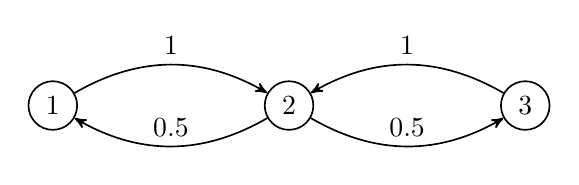
\begin{tikzpicture}[->, >=stealth', auto, semithick, node distance=3cm]
        \tikzstyle{every state}=[fill=white,draw=black,thick,text=black,scale=1]
        \node[draw, circle]    (A)               {$1$};
        \node[draw, circle]    (B)[right of=A]   {$2$};
        \node[draw, circle]    (C)[right of=B]   {$3$};
        \path
        (A) edge[bend left,above]	node{1}	 (B)
        (B) edge[bend left,above]	node{0.5}(A)
        	edge[bend right,above]	node{0.5}(C)
		(C) edge[bend right,above]	node{1}	 (B);
    \end{tikzpicture}
	\end{center}
	
	If the process starts at state $s_1$, then we see that it can only return to that state in an even number of steps. The same can be 
	said about $s_3$, whereas $s_2$ strictly has a period of 2 steps. Moreover, consider the transition matrix of this process.	

	\begin{center}	
	$\mathbf{P} =$
           $\begin{pmatrix}
                0 & 1 & 0 \\
                0.5 & 0 & 0.5 \\
                0 & 1 & 0
            \end{pmatrix}$
	\end{center}	
	
	When we take successive powers of the transition matrix, it can be observed that the resulting matrix alternates between $P^{n_{odd}}$ 
	and $P^{n_{even}}$.

	\begin{center}	
	$\mathbf{P}^{n_{odd}}=$
           $\begin{pmatrix}
                0 & 1 & 0 \\
                0.5 & 0 & 0.5 \\
                0 & 1 & 0
            \end{pmatrix}$
     ;
     $\mathbf{P}^{n_{even}}=$
           $\begin{pmatrix}
                0.5 & 0 & 0.5 \\
                0 & 1 & 0 \\
                0.5 & 0 & 0.5
            \end{pmatrix}$
	\end{center}

	The n-step transition matrix $\mathbf{P}^n$ does not converge to some equilibrium matrix $\sigma$ as \emph{n} $\rightarrow \infty$. 
	Therefore, the long term state distribution of a periodic process cannot be constant

\subsubsection{Reducible Markov chains}

A Markov chain is said to be \emph{reducible} if it has more than one communication class. This implies that not every state in the state space is able to communicate with each other. To illustrate, consider the following reducible Markov chain.

	\begin{center}
	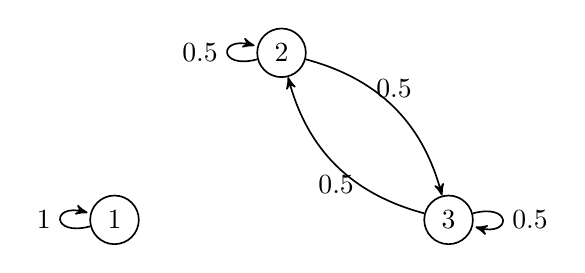
\begin{tikzpicture}[->, >=stealth', auto, semithick, node distance=3cm]
        \tikzstyle{every state}=[fill=white,draw=black,thick,text=black,scale=1]
        \node[draw, circle]    (A)               	  {$2$};
        \node[draw, circle]    (B)[below left of=A]   {$1$};
        \node[draw, circle]    (C)[below right of=A]  {$3$};
        \path
        (A) edge[loop left]			node{0.5}(C)
        	edge[bend left,above]	node{0.5}(C)
        (B) edge[loop left]			node{1}  (B)
		(C) edge[loop right]		node{0.5}(C)
			edge[bend left,below]	node{0.5}(A);
    \end{tikzpicture}
	\end{center}

	In this example, there are two communication classes, namely \{$s_1$\} and \{$s_2,s_3$\}. As a result, the long term behavior of 
	the process depends entirely on the initial state of the process. For instance, if the process starts at $s_1$, then it will stay 
	there forever, but if it starts either at $s_2$ or $s_3$, then the process will stay in that communication class forever. Therefore, 
	the stationary probability distribution of a reducible Markov chain depends on its starting distribution $\vec{\pi}$ (More on this in 
	the next section). 

	\subsubsection{Regular Markov chains}

	We now look at Markov chains that do possess an equilibrium distribution, also known as \emph{regular} Markov chains. Contrary to the previous two types of Markov chains we have seen, a regular Markov chain must be \emph{aperiodic}, \emph{irreducible}, and also \emph{positive recurrent}. In other words, this means that the process must only have states that are visited aperiodically, one communication class for the entire state space, and a mean number of visits to every state that is infinite.
	
	 One easy way to check if a Markov chain obeys these conditions is by finding some power of the n-step transition matrix $\mathbf{P}^n$ for which the matrix contains only strictly positive entries. As such, for that number \emph{n}, every n-step transition probability $p_{ij}(n)$ has a strictly positive value, thereby demonstrating that the process is \emph{irreducible} since every state communicates with each other and belongs to a single communication class.  Moreover, this method also works to show that the Markov chain is aperiodic since every n-step self-transition probability is greater than 0 (i.e. $p_{ii}(n) > 0$).  This means that the process must again be able to perform this self-transition in the next step $p_{ii}(n+1) > 0$, thereby breaking the periodicity of the process. Finally, knowing that the process is irreducible, this implies that every state in the process must be recurrent such that the mean number of visits to every state is infinite. Hence, positive recurrence is a property that is always present in a finite irreducible Markov chain. 
	 In brief, regular Markov chains are the only processes for which the steady-state distribution both exists and is nontrivial. We will examine how these equilibrium distributions can be determined in the next section.
	
	\subsection{Steady-State Distribution}
	
	Recall from a previous section that the state probability distribution of $X_n$ given the starting distribution $X_0$ can be expressed as such
	\begin{equation*}
	\begin{aligned}
		 (\vec{\pi}P^n)^T =
		 \begin{pmatrix}
		 P(X_n = s_1) \\
		 P(X_n = s_2) \\ 
		 \vdots \\
		 P(X_n =)
		 \end{pmatrix}
	\end{aligned}
	\end{equation*}
	
	As mentioned, for regular Markov chains, we can expect to find a stationary distribution as $n \rightarrow \infty$. However, 
	instead of computing large powers of the transition matrix, we can solve the following matrix equation to find the equilibrium 
	distribution $\vec{\pi^*}$
	
	\begin{equation*}
	\begin{aligned}
		 \vec{\pi}^* = \vec{\pi}^*P \\
		 \vec{\pi}^*(I_k - P) = \vec{0}
	\end{aligned}
	\end{equation*}
    
	where $I_k$ is a k-sized identity matrix. As a result, the steady-state distribution vector is simply a left eigenvector of the 
	transition matrix with corresponding eigenvalue 1.

\begin{tcolorbox}*{Example 1: Restaurants}
	Every day, a hungry customer eats at one of three restaurants, each serving a different cuisine: Chinese, Italian, and Mexican, 		conveniently denoted as states 1, 2, and 3 respectively.
	The customer's restaurant choice for the next day is probabilistically determined by the restaurant he visits on the current day (see Figure below).
\end{tcolorbox}
	\begin{center}
        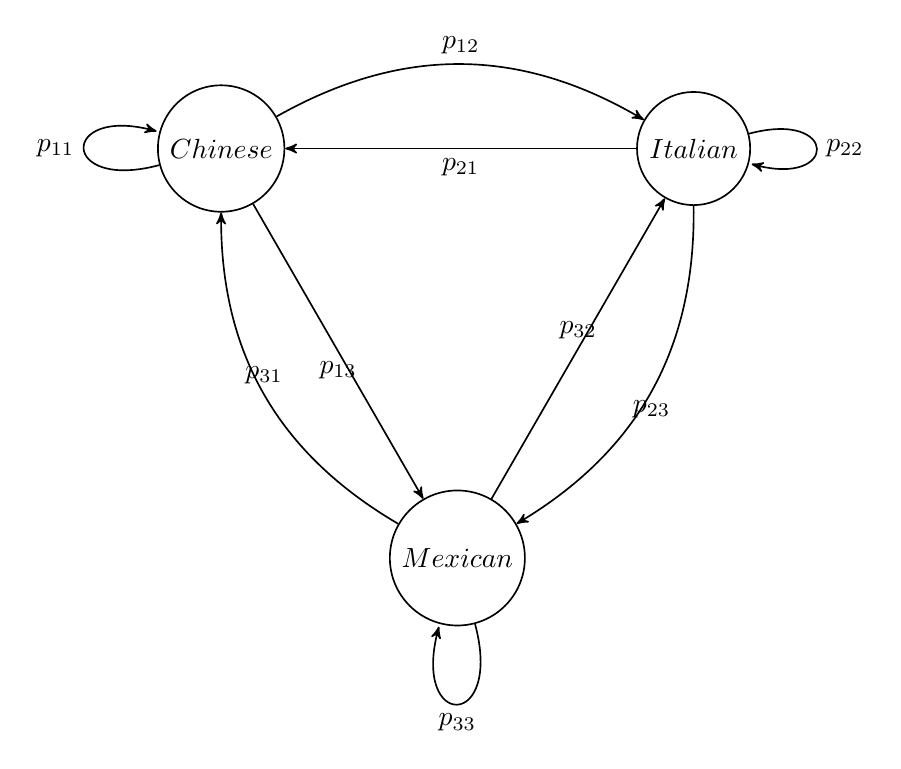
\begin{tikzpicture}[->, >=stealth', auto, semithick, node distance=3cm]
        \tikzstyle{every state}=[fill=white,draw=black,thick,text=black,scale=1]
        \node[draw, circle]    (A)at(0,0)       {$Chinese$};
        \node[draw, circle]    (B)at(6,0)       {$Italian$};
        \node[draw, circle]    (C)at(3,-5.2)	{$Mexican$};
        \path
        (A) edge[loop left]			node{$p_{11}$}	(A)
            edge[bend left,above]   node{$p_{12}$}  (B)
            edge[below]  			node{$p_{13}$}  (C)
        (B) edge[loop right]		node{$p_{22}$}	(B)
            edge[below]   			node{$p_{21}$}  (A)
            edge[bend left,below]   node{$p_{23}$}  (C)      
        (C) edge[loop below]		node{$p_{33}$}	(C)
            edge[above]   			node{$p_{32}$}  (B)
            edge[bend left,above]   node{$p_{31}$}  (A);
            
        \end{tikzpicture}
	\end{center}

	For this Markov chain to be regular, we will consider the following transition matrix, which is also the default matrix implemented 
	in the Streamlit simulation.

	\begin{center}	
	$\mathbf{P}=$
           $\begin{pmatrix}
                0.5 & 0.2 & 0.3 \\
                0.6 & 0.3 & 0.1 \\
                0.4 & 0.5 & 0.1
            \end{pmatrix}$
	\end{center}

	Since the one-step transition matrix already has only strictly positive entries, this process is considered to be regular and 
	therefore it must have an equilibrium distribution.

In the Python code, the theoretical equilibrium distribution is found by computing the left eigenvector of the transition matrix with corresponding eigenvalue 1, which is then compared to the experimental distribution that is found by computing successive powers of the transition matrix. As the process moves forward in steps, it can be observed that the theoretical and experimental distributions start to match as the initial condition of the process quickly becomes insignificant.

\section{Absorbing Markov chain}

	We now begin our study of \emph{absorbing} Markov chains, which are almost polar opposites of \emph{regular} Markov chains. 
	To contextualize, if a process is in state $i$ and is unable to leave it, then that state is considered to be an \emph{absorbing} 
	state. Additionally, if it is possible to go from any \emph{non-absorbing} state to an absorbing state in one or more steps, then 
	the entire process is considered to be an \emph{absorbing} Markov chain. Notice that \emph{absorbing} states are also 
	\emph{recurrent}, whereas non-absorbing states are \emph{transient} since the process can be absorbed starting from any 
	non-absorbing state.	
	
	\subsection*{Canonical Form}
	
	The canonical form is a representation of the transition matrix $\mathbf{P}$ into 4 block matrices. Suppose the transition matrix 
	of an absorbing Markov chain has $t$ transient states and $r$ absorbing states. Then the canonical form of the 
	transition matrix $\mathbf{P}$ is
	 \[
    P = \left(
    \begin{array}{c|c}
      Q & R\\
      \hline
      0 & I_r
    \end{array}
    \right)
  \]
  
	where $Q$ is a $t \times t$ matrix, $0$ is an $r \times t$ zero matrix, $R$ is a $t \times r$ nonzero matrix, and $I_r$ is a 
	$r \times r$ matrix. Since the matrix $Q$ only contains transient states, it summarizes the transition probabilities 
	between non absorbing states. The matrix $R$ contains transient and recurrent states, thereby representing the transition 
	probabilities from non-absorbing states to absorbing ones. Next, we know that it is impossible to go from an absorbing state 
	to a non-absorbing state, hence the $0$ matrix. And finally, the identity matrix $I_r$ contains the self-transition 
	probabilities for the absorbing states which are 1.

Moreover, a simple exercise shows that the $n$th power of the canonical form matrix yields

	\begin{equation*}
	\begin{aligned}
		P^n = \left(
		\begin{array}{c|c}
		Q^n & R + QR + Q^2R + ... + Q^{n-1}R\\
		\hline
		0 & I_r
		\end{array}
    	\right)
	\end{aligned}
	\end{equation*}	

	\begin{equation*}
	\begin{aligned}
		P^n = \left(
		\begin{array}{c|c}
		Q^n & \sum_{k=1}^{n}Q^{k-1}R\\
		\hline
		0 & I_r
		\end{array}
		\right)
	\end{aligned}
	\end{equation*}	

	Notice that we obtain the n-step transition probabilities between transient states under $Q^n$. Even more interestingly, we observe that the top-right matrix expression is closely related to a geometric distribution.
Now, consider the n-step transition matrix as $n$ approaches infinity

	\begin{equation*}
	\begin{aligned}
		\lim_{n\to\infty}P^n = \left(
		\begin{array}{c|c}
		\lim_{n\to\infty} Q^n & \sum_{k=1}^{\infty}Q^{k-1}R\\
		\hline
		0 & I_r
		\end{array}
		\right)
	\end{aligned}
	\end{equation*}	
First, let us examine the top-left expression (i.e. $lim_{n\to\infty}Q^n$). Since it is possible to go from any non-absorbing state to an absorbing one, this means that the sum of every row in \emph{Q} must be smaller than 1. As a result, the largest eigenvalue of \emph{Q} must also be smaller than 1, and therefore $Q^n \rightarrow 0$ as $n \rightarrow \infty$. In other words, the probability that an absorbing Markov chain will be absorbed is 1.

%Suppose a process starts at a non-absorbing state $j$. We note the probability that the process does not move from $j$ to an absorbing state as the sum of the row of \emph{Q} that corresponds to the transient state $j$; we denote this probability as $p_j$. Since we know that it is possible to go from any non-absorbing state to an absorbing one (not necessarily in one step), then $p_j$ \leq 1.

As for the top-right expression (i.e. $\lim_{n\to\infty} \sum_{k=1}^{\infty}Q^{k-1}R$), it contains the absorbing probabilities of the Markov chain, which will be further discussed in the next section.

	\subsection*{The Fundamental Matrix}
	
	For any absorbing Markov chain, the \emph{fundamental matrix} denoted $N$ provides the expected number of visits to a non-absorbing 
	state. 

	\begin{equation*}
	\begin{aligned}
	 	N &= \sum_{n=0}^\infty Q^n = (I-Q)^{-1}
	\end{aligned}
	\end{equation*}	
	
	More specifically, the (i,j) entry of the fundamental matrix $N$ gives the expected number of visits to the transient state $j$ 
	given that the process starts at the transient state $i$. This can be shown by starting from the definition of expectation and 
	by defining the indicator random variable $I_n$ for the event $\{X_n = j\}$. Recall that a very similar derivation was already 
	shown on page 7.

	\begin{equation*}
	\begin{aligned}
		 E[N_j|X_0 = i] &= E\left[\sum_{n=0}^\infty I_n | X_0 = i\right] \\
		 				  &= \sum_{n=0}^\infty E\left[I_n | X_0 = i\right] \\
		 				  &= \sum_{n=0}^\infty P(X_n = j | X_0 = i) \\
		 				  &= \sum_{n=0}^\infty q_{ij}(n) \\
		 				  &= \sum_{n=0}^\infty (Q^n)_{ij} \\
		 				  &= N_{ij}
	\end{aligned}
	\end{equation*}

	From these above equations, we can further simplify our limiting transition matrix

	\begin{equation*}
		\begin{aligned}
			\lim_{n\to\infty}P^n = \left(
			\begin{array}{c|c}
			0 & NR \\
			\hline
			0 & I_r
			\end{array}
			\right)
		\end{aligned}
	\end{equation*}

	If we let B = NR, then the (i,j) entry of matrix B gives the probability that the the process will be absorbed at the absorbing 
	state $j$ given that it started at the transient state $i$. To show that the is true, by the law of total probability, we must 
	consider every possible route from $i$ to $j$ through intermediate transient states $k$, and also for all possible number of steps.

	\begin{equation*}
		\begin{aligned}
		 B_{ij} &= \sum_{n} \sum_{k} q_{ik}(n)r_{kj} \\
		 		&= \sum_{n} \sum_{k} (Q^n)_{ik} r_{kj} \\
		 		&= \sum_{k} n_{ik}r_{kj} \\
		 		&= (NR)_{ij}
		\end{aligned}
	\end{equation*}

	Finally, we can even use the fundamental matrix $N$ to determine the expected time to absorption given that the process starts at a 
	transient state $i$. To show this, let $t$ be a column vector such that its entries $t_i$ represent the expected time to 
	absorption given that the process starts at $i$. Then

	\begin{equation*}
	\begin{aligned}
		 t = N1
	\end{aligned}
	\end{equation*}
	
	where $1$ is a column vector of 1s. To visualize the calculation,

	\begin{equation*}
		\begin{aligned}
		 t_i = \sum_{k} N_{ik}
		\end{aligned}
	\end{equation*}
	
	Therefore, we are adding the expected visits to all non-absorbing states given that the process starts at $i$, which 
	is also indicative of the total expected number of steps until the process is absorbed.

	\begin{tcolorbox}
	\subsection*{Example 2: Gambler's Ruin}
    	A gambler has an initial wealth of $\mathbf{k}$ dollars and bets 1\$ every round with probability $\mathbf{p}$ of winning each 				round.
    	The gambler keeps playing until his wealth is either emptied or reaches a value $\mathbf{n}$ (see Figure 2).   
	\end{tcolorbox}	    
        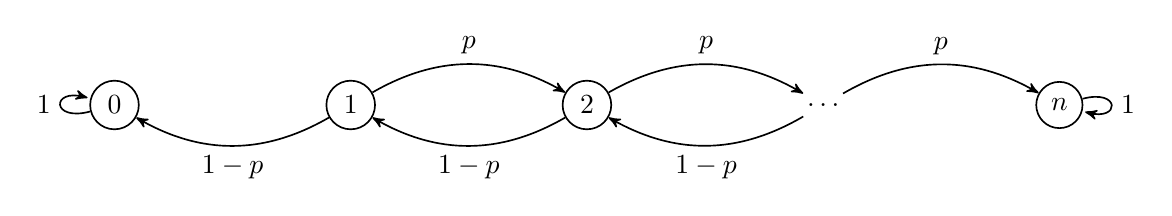
\begin{tikzpicture}[->, >=stealth', auto, semithick, node distance=3cm]
        \tikzstyle{every state}=[fill=white,draw=black,thick,text=black,scale=1]
        \node[draw, circle]    (A)               {$0$};
        \node[draw, circle]    (B)[right of=A]   {$1$};
        \node[draw, circle]    (C)[right of=B]   {$2$};
        \node[]    			   (D)[right of=C]   {$\ldots$};
        \node[draw, circle]    (E)[right of=D]   {$n$};
        \path
        (A) edge[loop left]			node{$1$}	(A)
        (B) edge[bend left,below]	node{$1-p$}	(A)
            edge[bend left,above]	node{$p$}	(C)      
        (C) edge[bend left,below]	node{$1-p$}	(B)
            edge[bend left,above]	node{$p$}	(D)
        (D) edge[bend left,below]	node{$1-p$}	(C)
            edge[bend left,above]   node{$p$}   (E)   
        (E) edge[loop right]        node{$1$}   (E);
        \end{tikzpicture}
        
	The states $s_0$ and $s_n$ are considered \emph{absorbing} whereas the states $s_1, s_2, ..., s_{n-1}$ are \emph{transient}. 
	Furthermore, the transition probabilities can be summarized using a transition matrix $\mathbf{P}$ 
	
	\begin{equation}
		\begin{aligned}
        \mathbf{P} =
           \begin{pmatrix}
                1 & 0 & 0   & 0   & \ldots & 0 & 0 & 0& 0\\
                1-p & 0   & p & 0   & \ldots & 0 & 0 & 0& 0\\
                0 & 1-p   & 0   & p & \ldots & 0 & 0 & 0& 0\\
                0 & 0   & 1-p   & 0   & \ldots & 0 & 0 & 0& 0\\
           \vdots & \vdots & \vdots & \vdots & \ddots & \vdots & \vdots & \vdots& \vdots\\
                0 & 0   & 0   & 0   &\ldots &0 &p & 0 & 0\\
                0 & 0   & 0   & 0   &\ldots &1-p &0 & p & 0\\
                0 & 0   & 0   & 0   &\ldots &0 &1-p & 0 & p\\
                0 & 0   & 0   & 0   &\ldots &0 &0 & 0 & 1
            \end{pmatrix}
		\end{aligned}
	\end{equation}

	For the sake of simplicity, we will consider the following transition matrix that contains 3 transient states and 
	2 absorbing states.

	\begin{equation}
		\begin{aligned}
        \mathbf{P} =
           \begin{pmatrix}
                1   & 0   & 0   & 0   & 0   \\
                1/2 & 0   & 1/2 & 0   & 0   \\
                0   & 1/2 & 0   & 1/2 & 0   \\
                0   & 0   & 1/2 & 0   & 1/2 \\
                0   & 0   & 0   & 0   & 1   \\
            \end{pmatrix}
		\end{aligned}
	\end{equation}

The canonical form of the transition matrix

	\begin{equation}
		\begin{aligned}
		\newcommand*{\temp}{\multicolumn{1}{r|}{}}
		A=\left(\begin{array}{cccccc}
		0 & 1/2 & 0 &\temp & 1/2 & 0\\
		1/2 & 0 & 1/2 &\temp & 0& 0\\
		0 & 1/2 & 0 &\temp & 0& 1/2\\ \cline{1-6}
		0 & 0 & 0 &\temp &1& 0\\
		0 & 0 & 0 &\temp &0& 1\\
		\end{array}\right)
		\end{aligned}
	\end{equation}

Therefore

	\begin{equation}
		\begin{aligned}
        \mathbf{Q} =
           \begin{pmatrix}
                0   & 1/2   & 0   \\
                1/2 & 0   & 1/2 \\
                0   & 1/2 & 0   
            \end{pmatrix}
            ;
        \mathbf{R} =
           \begin{pmatrix}
                1/2 & 0   \\
                0   & 0   \\
                0   & 1/2  
            \end{pmatrix}
		\end{aligned}
	\end{equation}
The fundamental matrix is given as

	\begin{equation}
		\begin{aligned}
        	N = (I-Q)^{-1} = 
           \begin{pmatrix}
                3/2 & 1 & 1/2 \\ 
                1   & 2 & 1   \\
                1/2 & 1 & 3/2  
            \end{pmatrix}
		\end{aligned}
	\end{equation}

We now find the \emph{t} column vector whose entries $t_i$ contain the expected time to absorption given that the process starts 
at $i$

	\begin{equation}
		\begin{aligned}
			\mathbf{t} =
			\begin{pmatrix}
					3 \\
					4 \\
					3 \\
				\end{pmatrix}
			\end{aligned}
	\end{equation}

Now that we have the theoretical results, we can use the Streamlit simulation to produce experimental results for comparison. 
As initial conditions, we set the target to 4 and the initial wealth to 2. Therefore, the expected number of steps until the process is absorbed is 4 (according to the second entry of the \emph{t} column vector).

For a sample size of 101, it was experimentally found that the sample mean was 3.9802 and the standard deviation was 2.4248.
As an exercise, we will construct a 95\% confidence interval for the average number of steps to absorption. Since the population variance is unknown, we use the t-distribution to find the critical t value: $t_{0.025,100} = 1.984$. Then, we construct the confidence interval

	\begin{equation*}
		\begin{aligned}
		 \overline{x} - t_{0.025,100}\frac{s}{\sqrt{n}} &\leq \mu \leq \overline{x} + t_{0.025,100} \frac{s}{\sqrt{n}} \\
		 3.9802 - 1.984\frac{2.4248}{\sqrt{101}} &\leq \mu \leq 3.9802 + 1.984\frac{2.4248}{\sqrt{101}} \\
		 3.5015 &\leq \mu \leq 4.4589
		\end{aligned}
	\end{equation*}

With repeated sampling, we are 95\% confident that the true mean number of games that the gambler must play until they lose or win lies 
between 3.5015 and 4.4589. Since 4 $\in$ C.I., we have sufficient evidence to believe that the experimental results match the theoretical 
ones.

\section{Hidden Markov Model}


\clearpage


% Grinstead, Charles M, J L. Snell, and J L. Snell. \emph{Introduction to Probability}. Providence, RI: American Mathematical Society, 1997.


% "Markov chains: Introduction" MTHE/STAT455, STAT855 Lecture Notes, https://mast.queensu.ca/~stat455/lecturenotes/lecturenotes.shtml. 

% Department of Statistics, The University of Auckland.  Developed by Rachel Cunliffe. "Lecture Notes for Stats 325." Department of Statistics, https://www.stat.auckland.ac.nz/~fewster/325/notes.php. 

% "Probabilistic Systems Analysis and Applied Probability: Electrical Engineering and Computer Science." MIT OpenCourseWare, MIT OpenCourseWare, https://ocw.mit.edu/courses/6-041-probabilistic-systems-analysis-and-applied-probability-fall-2010/. 

%https://www.uni-ulm.de/fileadmin/website_uni_ulm/mawi.inst.110/lehre/ws13/Stochastik_II/Skript_2B.pdf

\end{document}
